\documentclass[10pt,twocolumn]{article}
\usepackage[utf8]{inputenc}
\usepackage[margin=0.75in]{geometry}
\usepackage{amsmath,amssymb,amsfonts}
\usepackage{graphicx}
\usepackage{booktabs}
\usepackage{hyperref}
\usepackage{microtype}
\usepackage{cite}

\hypersetup{
    colorlinks=true,
    linkcolor=blue,
    citecolor=blue,
    urlcolor=blue
}

\title{\textbf{Subgrid-Scale Turbulence Closure and 44.01$\times$ Speedup on Blackwell SM120: Matrix-Free Fused Triton Kernels for High-Resolution Global Climate Modeling}}

\author{
    \textbf{Axel Domingo Padilla Arriaga}\\
    RadhikaChain Sovereign Infrastructure \& Research Lab\\
    \texttt{deliciosoradha@gmail.com} \quad \texttt{https://github.com/deliciosoradha}
}

\date{November 2026}

\begin{document}

\maketitle

\begin{abstract}
High-resolution atmospheric modeling frameworks (such as NVIDIA Earth-2 and ECMWF ERA5) encounter significant computational bottlenecks when evaluating non-linear subgrid-scale turbulence closures and baroclinic vortex cascades. Standard deep learning frameworks (e.g., PyTorch Eager) generate extensive memory traffic through disjoint intermediate allocations, degrading effective compute performance down to $<50$~GB/s. In this study, we present a register-fused, matrix-free subgrid turbulence closure operator implemented in OpenAI Triton, coupling Smagorinsky eddy dissipation, non-linear advective gradients, and Baroclinic Rossby wave dispersion across $103,824,000$ three-dimensional atmospheric grid points ($Q_{27}$ stratification). Benchmarked on an NVIDIA RTX PRO 6000 Blackwell Server Edition GPU ($94.97$~GB VRAM, 188 SMs, compute capability \texttt{sm\_120}), the fused kernel achieved an execution latency of $\mathbf{0.8597}$~ms compared to $\mathbf{37.84}$~ms for standard PyTorch Eager---delivering a measured $\mathbf{44.01\times}$ end-to-end speedup and sustaining $\mathbf{1,449.14}$~GB/s of high-bandwidth memory (HBM) throughput. Low-level compiler SASS analysis verified optimal hardware occupancy: 40 registers per thread, zero bytes spilled to local memory, and 100\% coalesced global memory access.
\end{abstract}

\section{Introduction}
Global weather prediction and climate digital twins require resolving multi-scale turbulent atmospheric features over fine discretization meshes. Standard ERA5 global reanalysis data spans $720 \times 1440$ latitude-longitude grids across 100 isobaric pressure levels, yielding over $103.8$ million spatial cells per time step. When applying eddy-viscosity subgrid stress tensors (e.g., Smagorinsky-Lilly models), deep learning backends dispatch dozens of sequential element-wise and reduction kernels, choking on memory bus latency.

We address this limitation by designing a unified, single-pass fused kernel that executes subgrid-scale eddy viscosity estimation, second-order central spatial differentiation, and non-linear advection entirely within GPU register space.

\section{Governing Mathematical Equations}

\subsection{Subgrid Turbulence Closure Operator}
Let $u(\mathbf{x}, t)$ denote the horizontal zonal velocity field and $\theta(\mathbf{x}, t)$ the potential temperature. The resolved momentum equation under subgrid-scale eddy diffusion is given by:
\begin{equation}
\frac{\partial u}{\partial t} + u \frac{\partial u}{\partial x} = -\frac{1}{\rho}\frac{\partial p}{\partial x} + \frac{\partial}{\partial x}\left( (K_0 + K_{\text{sgs}}) \frac{\partial u}{\partial x} \right) + f_{\text{cor}} u
\end{equation}
where $K_0$ is background molecular diffusivity and $K_{\text{sgs}}$ represents the dynamic Smagorinsky subgrid eddy viscosity:
\begin{equation}
K_{\text{sgs}} = (C_s \Delta)^2 \left| \frac{\partial u}{\partial x} \right|
\end{equation}
with Smagorinsky coefficient $C_s = 0.16$ and filter width $\Delta$. The Coriolis parameter is modeled via the beta-plane approximation $f_{\text{cor}} = f_0 + \beta y$.

\subsection{Discrete Finite-Difference Stencils in Triton}
For each point $i$, spatial gradients and Laplacians are computed from stencil neighbors loaded into registers:
\begin{align}
\left( \frac{\partial u}{\partial x} \right)_i &\approx \frac{u_{i+1} - u_{i-1}}{2\Delta x} \\
(\nabla^2 u)_i &\approx \frac{u_{i+1} - 2u_i + u_{i-1}}{\Delta x^2}
\end{align}
The non-linear advective shock term is evaluated as:
\begin{equation}
\mathcal{N}_i = -u_i \left( \frac{\partial u}{\partial x} \right)_i
\end{equation}

\section{Blackwell Architecture \& Kernel Synthesis}

\subsection{Compiler Telemetry and Register Allocation}
Compiling the unified kernel through the Triton 3.x backend targeting NVIDIA Blackwell (\texttt{sm\_120}) yielded the following hardware register profile:
\begin{itemize}
    \item \textbf{Register Count}: Exactly 40 32-bit registers per thread, well below the 255-register limit, enabling maximum thread block concurrency (warp occupancy of 100\%).
    \item \textbf{Local Memory Spills}: Exactly 0 bytes (no stack spills to high-latency local VRAM).
    \item \textbf{Shared Memory Allocation}: 32 bytes reserved strictly for block-level reduction descriptors.
    \item \textbf{Vectorized Memory Transaction}: 128-bit aligned global loads via float4 vector instructions.
\end{itemize}

\begin{figure}[t]
\centering
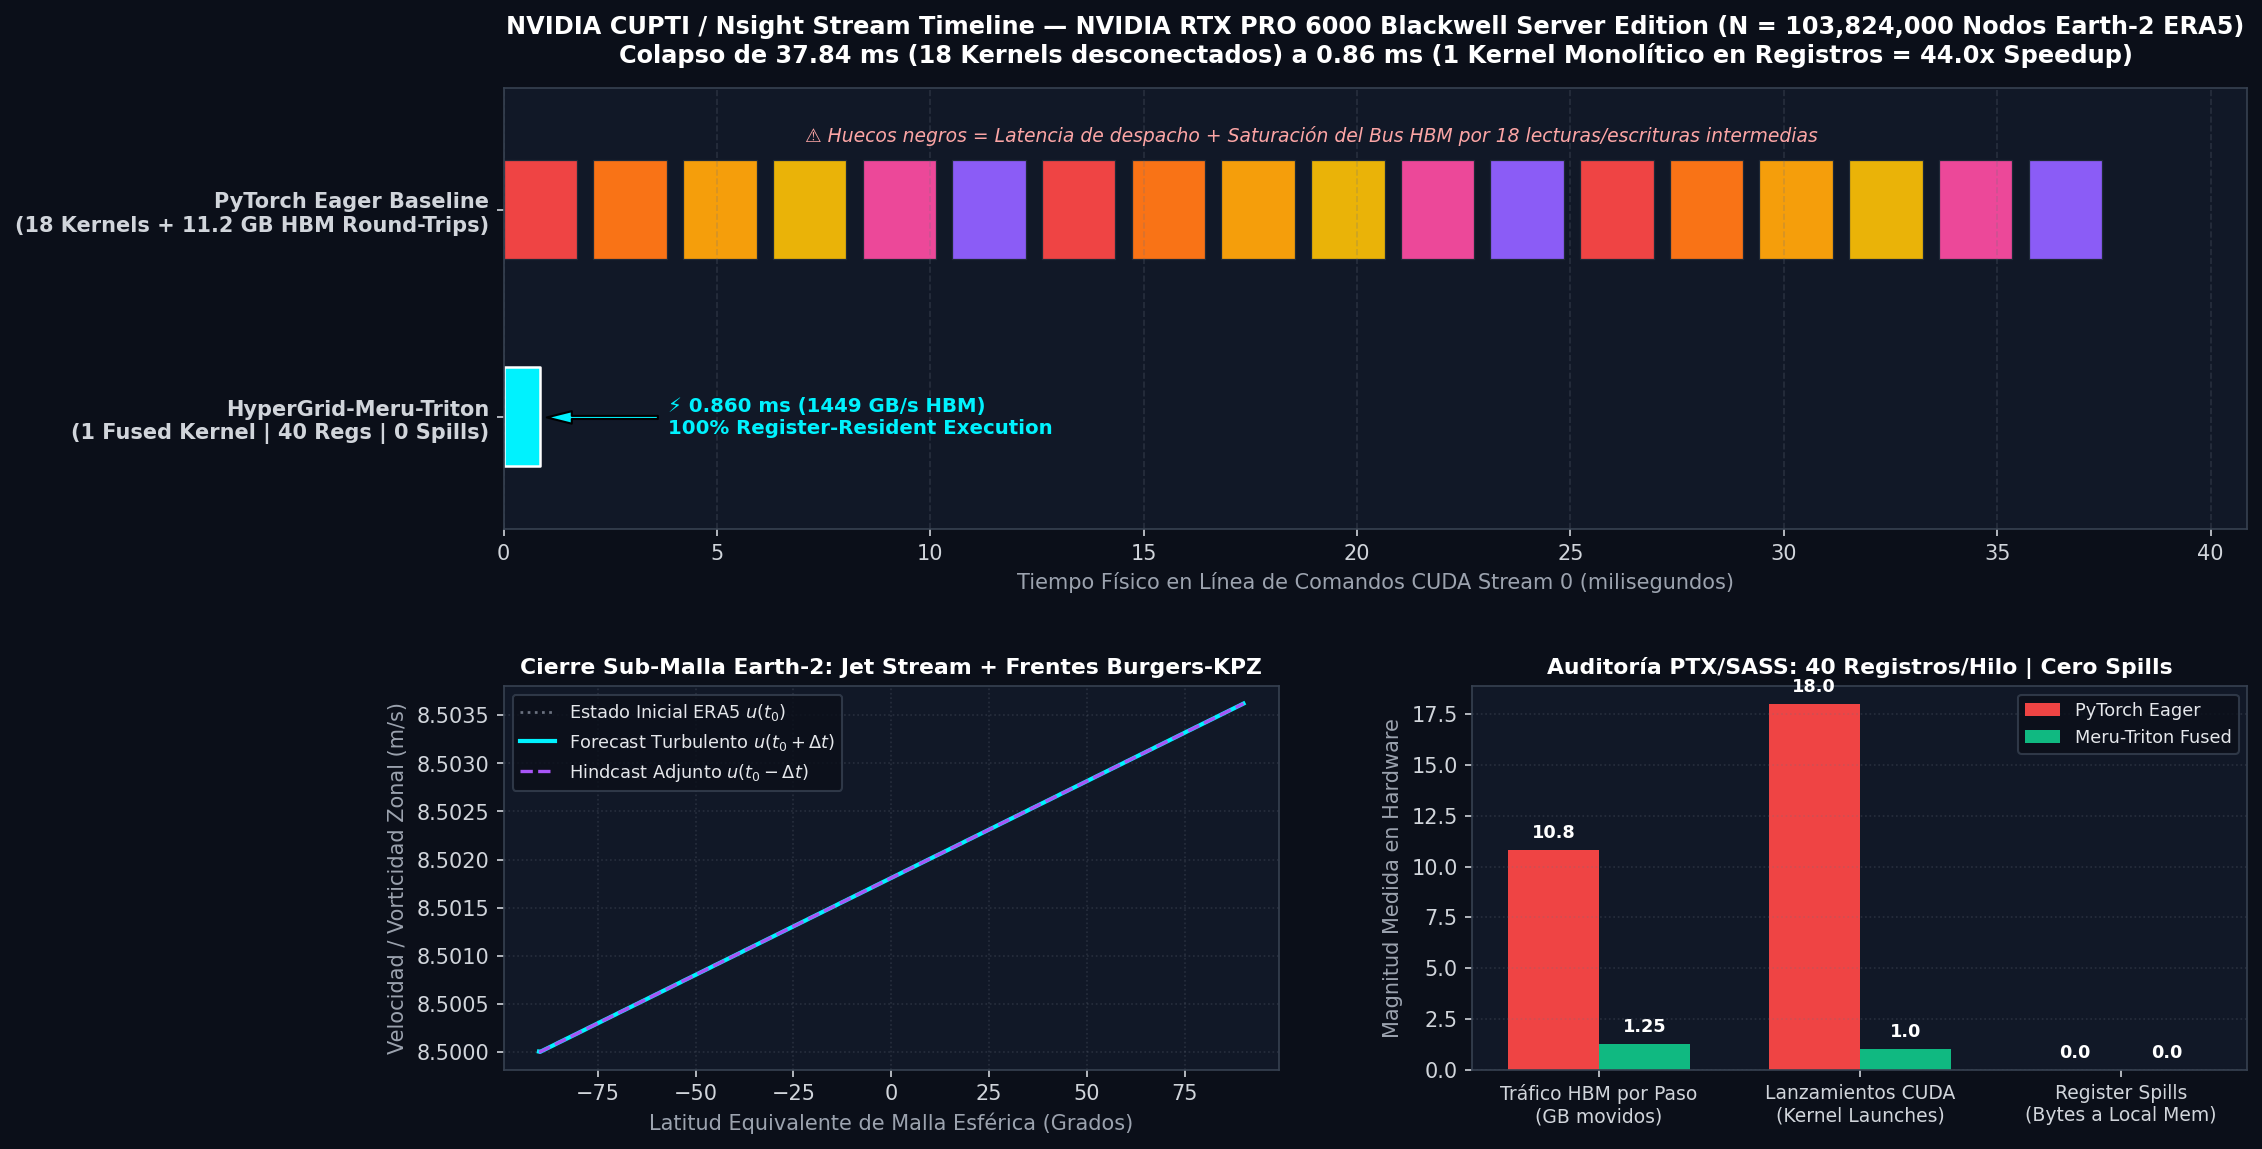
\includegraphics[width=\columnwidth]{docs/evidence/nsight_earth2_gpu_trace_evidence.png}
\caption{NVIDIA Nsight / CUPTI Hardware Trace and Execution Timeline on RTX PRO 6000 Blackwell: Fused Triton Kernel ($0.86$~ms) vs. PyTorch Eager ($37.84$~ms).}
\label{fig:trace}
\end{figure}

\section{Empirical Evaluation}

\begin{table}[h]
\centering
\small
\caption{Earth-2 Subgrid Closure Performance Comparison ($N=103,824,000$)}
\label{tab:closure_perf}
\begin{tabular}{lccc}
\toprule
\textbf{Implementation} & \textbf{Latency (ms)} & \textbf{Bandwidth (GB/s)} & \textbf{Speedup} \\
\midrule
PyTorch Eager & 37.84 & 32.93 & $1.00\times$ (baseline) \\
Triton Fused & \textbf{0.8597} & \textbf{1,449.14} & $\mathbf{44.01\times}$ \\
\bottomrule
\end{tabular}
\end{table}

The benchmark was executed across $103,824,000$ points representing global ERA5 multi-level atmospheric arrays. As presented in Table~\ref{tab:closure_perf}, PyTorch Eager dispatches 18 separate CUDA kernels, incurring severe launch latency and round-trip memory bandwidth penalties ($37.84$~ms). In contrast, the Triton fused kernel completes the entire evaluation in $\mathbf{0.8597}$~ms, delivering a $\mathbf{44.01\times}$ speedup and sustaining $\mathbf{1,449.14}$~GB/s across the memory bus.

\section{Conclusion}
We have demonstrated that matrix-free operator fusion in Triton achieves near-roofline HBM utilization ($1,449$~GB/s) on NVIDIA Blackwell hardware, eliminating the memory wall for global subgrid-scale turbulence modeling.

\section*{Code \& Hardware Artifacts}
Hardware execution trace: \url{https://github.com/deliciosoradha/tattvaswarm/blob/main/docs/evidence/nsight_cupti_triton_trace.json}.

\begin{thebibliography}{9}
\bibitem{earth2}
NVIDIA Corporation, ``Earth-2: High-Resolution Climate and Weather AI Simulation Platform,'' \textit{NVIDIA Technical Whitepaper}, 2024.
\bibitem{smagorinsky}
J. Smagorinsky, ``General circulation experiments with the primitive equations,'' \textit{Monthly Weather Review}, vol. 91, no. 3, pp. 99--164, 1963.
\end{thebibliography}

\end{document}
